\documentclass[twoside,openright,a4paper,papersize,uplatex,dvipdfmx]{jsarticle}
\usepackage[dvipdfmx]{graphicx,color}
\usepackage{mathtools}
\usepackage{physics}
% For hyper reference
\usepackage[dvipdfmx]{hyperref}
\usepackage{pxjahyper}

\newcommand{\rrr}{r} % symbol of risk/reward ratio

\begin{document}

  % \chapter{資金管理の理論} \label{chap: 資金管理の理論}
  \section{勝ちの平均回数と勝ちの確率} \label{sec: 勝ちの平均回数と勝ちの確率}

  あるアルゴリズムにしたがって$n$回トレードしたところ、勝ちトレードは$n^{+}$回であった。このとき勝ちの平均回数と勝ちの確率はそれぞれ
  \[
    \overline{ n^{+} } = \frac{ n^{+} }{ n }
      \qcomma
    p = \frac{ \expval{ n^{+} } }{ n }
  \]
  となる。ここの$ \expval{ n^{+} } $は$ n $回トレードした時に出る勝ち回数の期待値である。

  私たちが実際に観測するのは左側の勝ちの平均回数で、右の勝ちの確率はアルゴリズムに特有なものである。また勝ち平均回数は試行するたびに値が変動するのに対し、勝ち確率はトレードのどの時点でも定数である。

  例えば、ジョーカーを除いた52枚のトランプの組からランダムに1枚引いて、それがスペードであれば勝ち、というゲームを考える。引いたカードは元に戻し、シャッフルしてまた1枚引くことを繰り返す(抜いたものは抜いたままにしない)。このとき、もちろん$p = 1 / 4 = 0.25$である。この試行を100回やることを考えたならば、スペードが出て勝つ回数は$\expval{ n^{+} } = p n = 25$と期待される。しかし実際には100回目までで31回の勝ちが出たとする。このとき$n^{+} = 31$で$\overline{ n^{+} } = 31 / 100 = 0.31$となる。また、次の101回目を引いたとき$\overline{ n^{+} }$の値は変化するだろうが、$p$は$0.25$のまま変わることはない。

  $p$の値がわからない場合、我々がやるのは、大きな$n$で$n^{+}$をカウントし、$\overline{ n^{+} }$を$p$の代わりとして使っている。つまり
  \[
    p = \lim_{n \to \infty} \overline{ n^{+} }
  \]
  であるが現実には$n \to \infty$は不可能なため、$n \gg 1$で
  \[
    p \approx \overline{ n^{+} }
  \]
  として$p$の値を推定している。当たりが何本入っているかわからないくじ引きで$p$の値を知りたければ、何回も引いて当たりの平均回数を調べることになる。

  「勝率」という言葉が勝ちの平均回数を指しているのか、勝ちの確率を指しているのか曖昧な時がある。現実世界のことを考えているならば勝ちの平均回数、理論的な話をしているのであれば勝ちの確率、と頭を切り替えるのが必要である。「勝率$p$で…」という文があった場合、$\overline{ n^{+} }$の値を計算して、それを$p$の値と推測して使う。

  \subsection{オッズ} \label{subsec: オッズ}
  勝ち確率$p$の別表現としてオッズというものがある。オッズ$q$は失敗の確率を成功の確率で割ったもの。
  \[
    q = \frac{ 1 - p}{ p }
      \qq{or}
    q = \frac{ n^{-} }{ n^{+} }.
  \]
  オッズは$0 \le q < \infty$となり、値が小さいほど成功確率が高いことになる。

  \section{平均利益と利益の期待値} \label{sec: 平均利益と利益の期待値}
  $n^{+}$回の勝ちトレードに$i = 1, \ldots, n^{+}$とナンバリングし、それぞれの利益を$x_{i}^{+}$とする。このとき平均利益は
  \[
    \overline{ x^{+} } = \frac{1}{ n^{+} } \sum_{i = 1}^{ n^{+} } x_{i}^{+}
  \]
  となる。一方で、$x^{+}$の利益が得られる勝ち確率を$p \qty( x^{+} )$とすれば、一回当たりの利益の期待値は
  \[
    \expval{ x^{+} } = \sum_{ ^{\forall} x^{+}} p \qty( x^{+} ) x^{+}
    \qq{or}
    \expval{ x^{+} } = \int p \qty( x^{+} )  x^{+} \dd{ x^{+} }
  \]
  となるだろう。左は$x^{+}$が離散型確率変数の場合で、右は連続型の場合。

  例で理解してみよう。前節トランプの例で、スペードが出たらそのカードの数字と同じ額のお金がもらえるという設定にする。1回の勝ちでもらえる報酬の期待値は
  \[
    \expval{ x^{+} } = \frac{1}{13} \qty( 1 + 2 + \cdots + 13 ) = 7
  \]
  である。実際に10回試行したところ、勝ちは3回でてその報酬は3, 10, 4であったとする。この時の平均利益は
  \[
    \overline{ x^{+} } = \frac{3 + 10 + 4}{3} = 5.\dot{6}
  \]
  となる。

  平均損失$\overline{ x^{-} }$と損失の期待値$\expval{ x^{-} }$も同様に計算できる。ただし損失にはマイナスを含めて、$x_{i}^{-} \le 0$として扱うことにしよう。損益がゼロだったものは損失としてカウントする。

  \section{損益比率} \label{sec: 損益比率}
  次の量を損益比率(risk/reward ratio, RRR)という。
  \[
    \rrr = \abs{
      \frac{ \overline{ x^{+} } }{\overline{ x^{-} }}
    }
    \qq{or}
    \rrr = \abs{
      \frac{ \expval{ x^{+} } }{\expval{ x^{-} }}
    }.
  \]

  最も良いトレードは$p$と$\rrr$がともに大きいもので、最悪なのはともに小さいものである。また片方が小さくてももう片方が大きければ、安定して利益を出せることもある。

  勝率$p$が大きくて損益比率$\rrr$が小さければ、ちょこちょこと利益を生み出し、ごくたまにドカンと損失を喰らう。しかしトータルで見れば収益はプラスになっていることも考えられる。逆に勝率$p$が小さくて損益比率$\rrr$が大きければ、ちょこちょこと負け続けるものの、たまにドカンと一気に勝つことで収益がプラスになることが考えられる。

  \section{バルサラの破産確率} \label{sec: バルサラの破産確率}
  現在使っているアルゴリズムやトレード方法を続けた場合、最終的に破産(資金がゼロになる)確率をバルサラは計算した。この破産確率を知ることで、トレーディング方法を変更すべきかを決定できるようになる。

  %1枚の画像
  \begin{figure}[htbp]
    \centering
    
\includegraphics[width=120mm]{./fig/81011344.jpg}
    \caption{トレードする前から破産する確率は決まっている}
    \label{fig: お前はもう死んでいる}
  \end{figure}

  今までお金の変数を$x$としていたが、ここでは$m$とする(数列の添字が$x$なのは気持ち悪いため)。

  \subsection{簡単な例}
  \label{subsec: 簡単な例}
  あるゲームを考える。自分と相手(市場)の2人でやるゲームで、自分が勝てば相手から$1$のお金をもらい、負ければ相手に$1$のお金を支払う。つまり$\expval{ m^{\pm} } = \pm 1 \qc \rrr = \abs{1 / -1} = 1$とする。自分の勝つ確率は$p$で、負ける確率は$1 - p$であるとする。ただし大事な仮定として$p > 1/2 \qc q = (1 - p) / p < 1$とする。自分のはじめの所持金は$m_{0}$とする。自分の資金が$0$か$M \gg 1$になったらゲームを終了する。

  簡単のため$\expval{ m^{\pm} } = \pm 1$としているが、別に$\pm 1$でなくてもいい。$\expval{ m^{\pm} } = \pm k \neq 0$のときはお金の次元を持つ量をすべて$\abs{k}$で割り規格化すれば$\expval{ m^{\pm} } = \pm 1$の問題に帰着できる。とにかく$\rrr = 1$であればいい。

  自分の所持金が$m$のとき、最終的に資金が$0$になってゲームを終える確率$Q_{m}$を求めよう。

  境界条件としては
  \begin{align}
    Q_{0} = 1 \qc Q_{M} = 0. \label{eq: boundary_cond}
  \end{align}
  $Q_{m}$は過去の過程によらない。むしろ次のゲームの結果が勝ちか負けるかによっている。
  \begin{align*} % \label{eq: seq_2021-09-19}
    Q_{m} = p Q_{m+1} + \qty(1 - p) Q_{m - 1},
  \end{align*}
  整理して
  \begin{align} \label{eq: 2021-09-28-18-33}
    p Q_{m+1} - Q_{m} + \qty(1 - p) Q_{m - 1} = 0.
  \end{align}
  これは$m$に関する数列$\qty{Q_{m}}$の漸化式で、
  \begin{align} \label{eq: recurrent}
    Q_{m+2} - \alpha Q_{m+1} =
    \beta \qty( Q_{m+1} - \alpha Q_{m})
  \end{align}
  の形に変形できる。この$\alpha \qc \beta$は特性方程式
  \begin{align} \label{eq: quadratic_2021-09-19}
    p x^{2} - x + (1 - p) = 0
  \end{align}
  の解である。式(\ref{eq: recurrent})で$R_{m} = Q_{m+1} - \alpha Q_{m}$とおくと
  \begin{align*}
    R_{m} &= \beta R_{m-1} = \beta^{2} R_{m-2} = \cdots = \beta^{m} R_{0}
    = \beta^{m} \qty( Q_{1} - \alpha Q_{0} )
    = \beta^{m} \qty( Q_{1} - \alpha ).
  \end{align*}
  ただし式\eqref{eq: boundary_cond}の$Q_{0} = 1$を用いた。よって
  \begin{align} \label{eq: recurrent_2021-09-19-22-35}
    Q_{m} &= Q_{m-1} + \beta^{m-1} \qty( Q_{1} - \alpha ) \notag \\
    &= Q_{m-2} + \beta^{m-2} \qty( Q_{1} - \alpha ) + \beta^{m-1} \qty( Q_{1} - \alpha ) \notag \\
    &= \cdots \notag \\
    &= Q_{0} + \qty( Q_{1} - \alpha ) \sum_{k = 0}^{m-1} \beta^{k} \notag \\
    &= 1 + \qty( Q_{1} - \alpha ) \frac{1 - \beta^{m}}{1 - \beta}
  \end{align}
  となる。ところで式\eqref{eq: quadratic_2021-09-19}を解くと$x = 1 \qc q$となるが、$\beta = 1$とすると式\eqref{eq: recurrent_2021-09-19-22-35}の分母が$0$になり不定になる。よって$\alpha = 1 \qc \beta = q = \qty(1 - p) / p$を採用して、
  \begin{align*}
    Q_{m} = 1 + \qty(Q_{1} - 1) \frac{1 - q^{m}}{1 - q}.
  \end{align*}
  $Q_{1}$はこの式で$m = M$として求める。式\eqref{eq: boundary_cond}から$Q_{M} = 0$なので
  \begin{align*}
    0 = 1 + \qty(Q_{1} - 1) \frac{1 - q^{M}}{1 - q}
    \qc
    Q_{1} -1 = \frac{1 - q}{q^{M} - 1}
  \end{align*}
  となる。さらに、いま$p > 1/2 \qc q = (1 - p) / p < 1$を仮定しているので、$M \gg 1$のとき$q^{M} \approx 0$である。以上より、求めていた破産確率は
  \begin{align*}
    Q_{m} = \frac{q^{m} - q^{M}}{1 - q^{M}} \approx q^{m} = \qty( \frac{1 - p}{p} )^{m}
  \end{align*}
  となる。

  \subsection{より一般の場合}
  \label{subsec:より一般の場合}
  次に$\rrr \neq 1$すなわち$\expval{m^{+}} \neq \abs{\expval{m^{-}}}$の場合を考える。このときお金全体を$ L = \abs{ \expval{ m^{-} } }$の値で割り($m ' = m / \abs{ \expval{ m^{-} } }$)規格化のようなことをすることで、$\expval{ m'^{+} } = \rrr \qc \expval{ m'^{-} } = -1$と取り替えることができる。前節\ref{subsec: 簡単な例}と同様に漸化式を立てると
  \begin{align*}
    Q_{m'} = p Q_{m' + \rrr} + \qty(1 - p) Q_{m'-1}
  \end{align*}
  となり、整理して
  \begin{align} \label{eq: 2021-09-28-18-42}
    p Q_{m' + \rrr} - Q_{m'} + \qty(1 - p) Q_{m'-1} = 0.
  \end{align}

  さて前節\ref{subsec: 簡単な例}では式\eqref{eq: 2021-09-28-18-33}を解くのに特性方程式\eqref{eq: quadratic_2021-09-19}をたて、その解が$x = 1 \qc q$であったことから最終的な解は$Q_{m} = q^{m}$と得られた。このこととのアナロジーで式\eqref{eq: 2021-09-28-18-42}を解くには特性方程式
  \begin{align} \label{eq: 2021-09-28-18-56}
    p x^{1 + \rrr} - x + \qty(1-p) = 0
  \end{align}
  をたて、その$0 < x < 1$を満たす解$x = \sigma$が存在するならば漸化式\eqref{eq: 2021-09-28-18-42}の解は
  \begin{align} \label{eq: 2021-09-28-20-26}
    \sigma^{m' + 1} < Q_{m'} \le  \sigma^{m'}
  \end{align}
  となるらしい。$m' \qc r$が整数のときは$Q_{m'} = \sigma^{m'}$となるらしい。

  なぜそうなるのかは正直よくわかっていない。\href{http://geolog.mydns.jp/www.geocities.jp/y_infty/management/bankruptcy.html}{このWebページ}によると、\href{https://www.kinokuniya.co.jp/f/dsg-01-9784314000161}{確率論とその応用 〈1 下〉}という本に載っているらしい。まぁ、たしかに$Q_{m}$は確率だから$0 \le \sigma \le 1$で、$Q_{m}$の境界条件を考えると$\sigma = 0 \qc 1$となるのはまずい。$\sigma$が$0 < \sigma < 1$と式\eqref{eq: 2021-09-28-18-56}を満たすとするならば、たしかに$Q_{m} = \sigma^{m}$は式\eqref{eq: 2021-09-28-18-42}を満たす。$\rrr \ge 0 \qc \rrr \neq 1$としか与えられてないので、式\eqref{eq: 2021-09-28-18-56}は解析的には解けず、\href{https://ja.wikipedia.org/wiki/%E3%83%8B%E3%83%A5%E3%83%BC%E3%83%88%E3%83%B3%E6%B3%95}{ニュートン法}などで数値的に求めることになるだろう。

  破産の撤退ラインを$m' = 0$としていたが、$m' = m'_{\mathrm{ruin}}$で破産とするならば、式\eqref{eq: 2021-09-28-20-26}を
  \begin{align*}
    \sigma^{ \qty(m' - m'_{\mathrm{ruin}}) + 1} < Q_{m'} \le  \sigma^{m' - m'_{\mathrm{ruin}} }
  \end{align*}
  とすればよい。さらに$m' = m / \abs{\expval{m^{-}}} = m / L$であったので、もとの表式に戻すならば
  \begin{align*}
    \sigma^{
      \frac{
        m - m_{ \mathrm{ruin} }
      }{
        L
      } + 1
    } < Q_{m} \le \sigma^{
      \frac{
        m - m_{\mathrm{ruin}}
      }{
        L
      }
    }
  \end{align*}
  となる。

  \subsection{許容リスクを考慮に入れた場合} \label{subsec: 許容リスクを考慮に入れた場合}
  許容リスク(maximum risk)というものを導入する。許容リスクを$e$(ただし$0 < e < 1$)として、資金が$m$の時は$em$を賭ける。ゲームに勝てば$\rrr em$を得て、負ければ$em$を失う。資金は、勝てば$m + \rrr em = \qty(1 + \rrr e) m$となり、負ければ$m - em = \qty(1 - e) m$となる。つまり1回勝てば$\qty(1 + \rrr e)$倍、1回負ければ$\qty(1 - e)$倍になる。

  初めの資金を$m_{0}$とし、撤退ラインを$m_{\mathrm{ruin}} \neq 0$とする($m_{\mathrm{ruin}} = 0$だと無限に小さな資金を賭け続けることができてしまい、現実的ではない)。$n^{+}$回勝って$n^{-}$回負け、破産となる条件は
  \begin{align*}
    \qty(1 + \rrr e)^{ n^{+} } \qty(1 - e)^{n^{-}}  m_{0} \le m_{\mathrm{ruin}}
  \end{align*}
  となる。両辺の対数をとって
  \begin{align} \label{eq: 2021-09-28-22-29}
    n^{+} \log( 1 + \rrr e ) + n^{-} \log(1 - e) + \log(\frac{m_{0}}{m_{\mathrm{ruin}}}) \le 0.
  \end{align}
  $1-e < 1$であるから$\log(1 - e) < 0$であることに注意。ここで
  \begin{align*}
    M^{+} = \log( 1 + \rrr e )  \qc
    M^{-} = \log(1 - e) < 0 \qc
    M_{0} = \log(
      \frac{
        m_{0}
      }{
        m_{\mathrm{ruin}}
      }
    )
  \end{align*}
  とすると式\eqref{eq: 2021-09-28-22-29}は
  \begin{align*}
    n^{+} M^{+} + n^{-} M^{-} + M_{0} \le 0
  \end{align*}
  となる。これは、初期投資$M_{0} \qc$撤退ライン$0$で、勝てば$\expval{ m^{+} } = M^{+} \qc$負ければ$\expval{ m^{-} } = M^{-} < 0 $を得るゲームにおいて破産確率を求める問題に帰着する。すなわち$\rrr \neq 1$の前節\ref{subsec:より一般の場合}の問題に帰着する。

  \subsection{破産確率を求める手順まとめ} \label{subsec: 破産確率を求める手順まとめ}
  \begin{enumerate}
    \item 次の数値を設定、あるいはこれまでのトレードの成績から算出する。
    \begin{itemize}
      \item 初期投資$m$
      \begin{itemize}
        \item これは「現在の資金」とも解釈できる。つまり今が何回目の試行であれ、現在がゼロ回目の試行と捉え直すと、現在の資金は初期投資になる($m_{0} = m$)。
      \end{itemize}
      \item 撤退ライン$m_{\mathrm{ruin}} \neq 0$
      \item 勝ち確率あるいは勝率$p$
      \item 1回の勝ち負けの損益$\expval{m^{\pm}}$あるいは損益比率$\rrr$
      \item 許容リスク$0 < e < 1$
    \end{itemize}
    \item 次の量を計算する。
    \begin{align*}
      M^{+} = \log( 1 + \rrr e )  \qc
      M^{-} = \log(1 - e) < 0 \qc
      M = \log(
        \frac{
          m
        }{
          m_{\mathrm{ruin}}
        }
      )
    \end{align*}
    \item これを使って新しい損益比率$R = M^{+} / \abs{M^{-}} = - M^{+} / M^{-}$を計算する。
    \item 次の方程式をたて、$0 < \Sigma < 1$となる解$\Sigma$を(数値的に)求める。
    \begin{align*}
      p x^{1 + R} - x + \qty(1 - p) = 0.
    \end{align*}
    \item 破産確率$Q$は次の範囲にある。
    \begin{align*}
      \Sigma^{1 - M / M^{-}} < Q \le \Sigma^{- M / M^{-}}.
    \end{align*}
  \end{enumerate}

  \subsection{破産確率の解釈の仕方} \label{subsec: 破産確率の解釈の仕方}
  勝率$p \qc$損益比率$\rrr \qc$許容リスク$e$の値のバランスが大事だと一般的に言われている。
  特に許容リスクは$e = 2\%$より大きくしてはいけないと言われている。また破産確率は$Q \le 1\%$に収めるべきで、それより大きくなれば分析手法、トレーディング手法を再考すべきと言われている。

  \subsection{バルサラの破産確率表} \label{subsec: バルサラの破産確率表}
  「バルサラの破産確率表」とインターネットで計算すると、色々出てくる。しかし許容リスクを明示していないサイトがあるので注意。図\ref{fig: バルサラの破産確率表}は許容リスクが$e = 0.02$のときの破産確率表である。これを見ると、$Q = 100\%$から$Q = 0\%$への変化が急であることがわかる。

  %1枚の画像
  \begin{figure}[htbp]
    \centering
    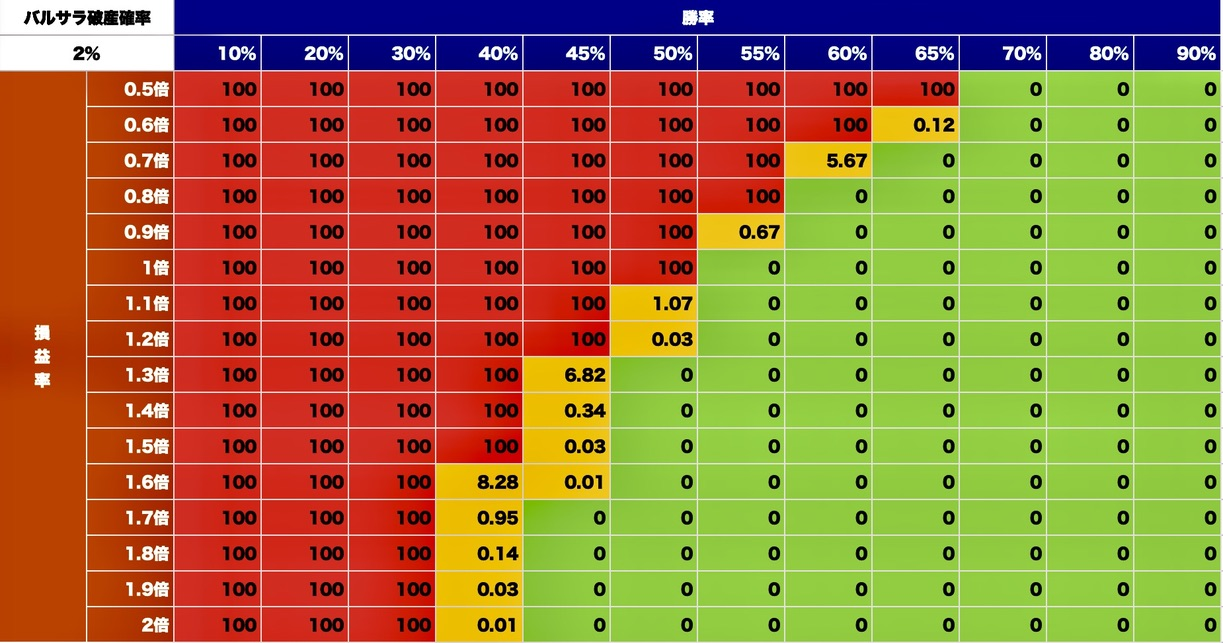
\includegraphics[width=120mm]{./fig/16A80743-B572-44E1-ACA1-136F844176C1_1_105_c.jpeg}
    \caption{バルサラの破産確率表の例($e = 0.02$)}
    \label{fig: バルサラの破産確率表の例}
  \end{figure}

  \bibliography{http://geolog.mydns.jp/www.geocities.jp/y_infty/management/bankruptcy.html}
\end{document}
